\subsubsection{Electric Technic Mini-Motor 9v (ID: 71427)}
\begin{figure}[H]
  \centering
  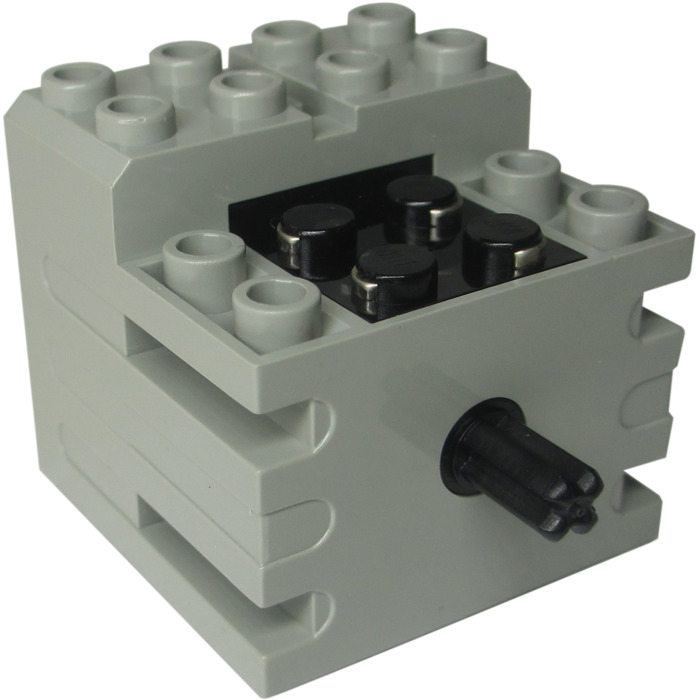
\includegraphics[width=3cm]{images/techAnalysis/LegoTechnicMiniMotor.jpg}
  \caption{LEGO Technic Mini-Motor 9v \cite{BrickOWl-figure-Technic-MiniMotor9v}}\label{fig:sssec:TechnicMiniMotor}
\end{figure}
This motor, shown in \autoref{fig:sssec:TechnicMiniMotor}, is an older motor for the LEGO Technic universe.
According to Philippe Hurbain, it is not as powerful as EV3 or NXT 2.0 motors, but with its 360rpm, it is faster than those motors.
And unlike the previously described servomotors, this motor does not feature a built-in rotation sensor and therefore does not allow for precise control in terms of degrees.
The motor is powered by an electric wire plate, attached to the top of the motor on the black square.
There exists an adapter cable which allows for the motor to plug-in to an RJ12 port, allowing the motor to be connected to both the EV3 and NXT 2.0 brick by default, which was tested during this analysis.
\cite{hurbain_lego_technicmotorComp}
